\section{Functional specifications}

\subsection{User interfaces}
In this subsection we will present all functional specifications of the user interfaces
included in the different aspects of our product.

\subsubsection{Mobile application}
The main user interface will be the Mobile application, it will reflect all necessary
data that could be useful for the user and for any data analysis required. \\
The landing page will display buttons to give, to the user, access to all the sensor
data as well as the plant's profile. Through the help of graphics the data from
the sensors will be displayed as it is, and more graphs will show data history and
offer some analysis such as a calendar to maintain a proper watering schedule for instance. \\
Some example of the final app display are as follows:

\begin{figure}
    \centering
    \begin{subfigure}[b]{0.3\columnwidth}
        \centering
        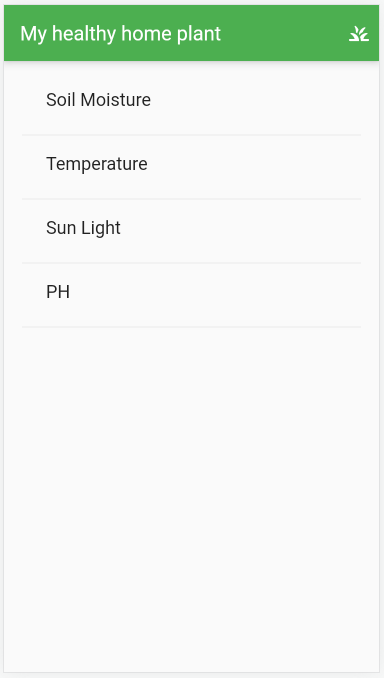
\includegraphics[width=\textwidth]{images/landing.png}
        \caption{Landing page}
    \end{subfigure}
    \begin{subfigure}[b]{0.3\columnwidth}
        \centering
        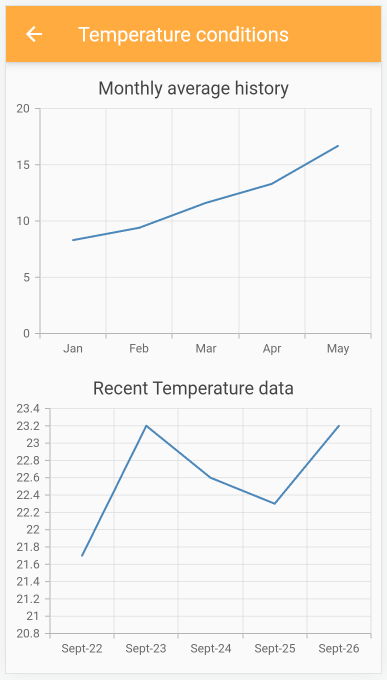
\includegraphics[width=\columnwidth]{images/temperature.png}
        \caption{Temperature}
    \end{subfigure}
    \\
    \begin{subfigure}[b]{0.3\columnwidth}
        \centering
        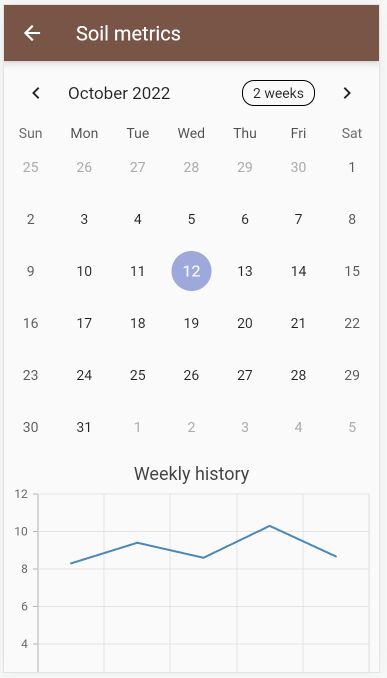
\includegraphics[width=\textwidth]{images/soil.png}
        \caption{Soil}
    \end{subfigure}
    \begin{subfigure}[b]{0.3\columnwidth}
        \centering
        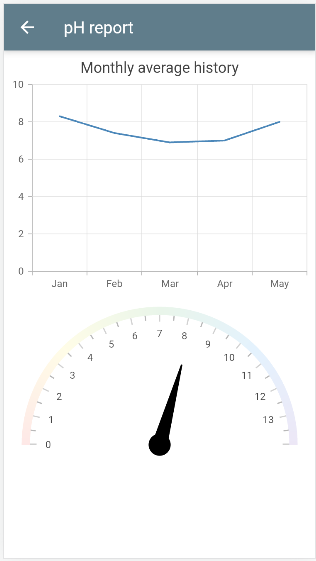
\includegraphics[width=\columnwidth]{images/pH.png}
        \caption{pH Page}
    \end{subfigure}
    \caption{Examples of displayed data from sensors}
    \label{fig:Examples of Displayed Data}
\end{figure}

The plant profile will exhibit an overview of the plant's current state in relation
to the previously set thresholds. It is also from this page that the user will be
able to manually update and modify the thresholds as well as editing the profile's
information. Through the share button users will be able to exchange plant data
and threshold settings. 

\begin{figure}[!ht]
    \centering
    \begin{subfigure}[b]{0.3\columnwidth}
        \centering
        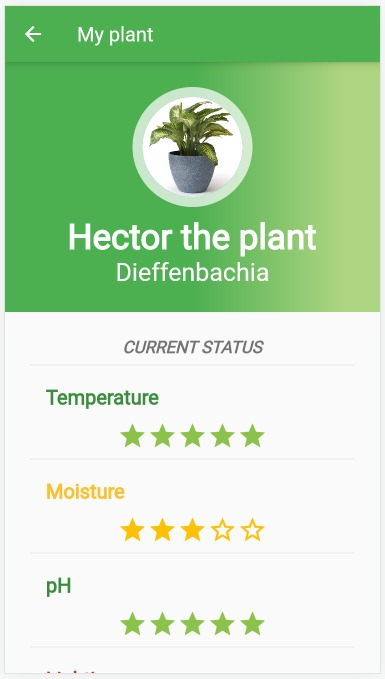
\includegraphics[width=\textwidth]{images/profile1.jpeg}
        \caption{Plant status}
    \end{subfigure}
    \begin{subfigure}[b]{0.3\columnwidth}
        \centering
        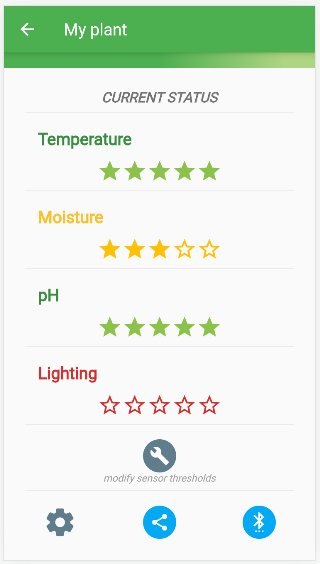
\includegraphics[width=\columnwidth]{images/profile2.png}
        \caption{Profile settings}
    \end{subfigure}
    \caption{Plant Profile Page}
    \label{fig:Plant Profile Page}
\end{figure}

\subsubsection{Physical device}
%TODO: Add if there are any buttons, leds that display a pairing mode or bluetooth connection?

Most plants like a soil with a pH between 6.0 and 7.5. If the soil is not acidic
enough for a crop, nutrients may be present in the soil, but the plant will not
be able to absorb them properly. The acidity of a soil is determined by the amount
of limestone it contains. The more limestone a soil contains, the more alkaline it is;
conversely, the less limestone it contains, the more acidic it is. This measure
will be satisfied with a \textbf{pH sensor}. \\
The ideal temperature for an indoor plant is between 15 and 19°C. It is important
to maintain a constant atmosphere throughout the day. In order to meet this requirement,
the device will incorporate a \textbf{temperature sensor}. \\
Most plants need a minimum amount of light in order to carry out the process of
photosynthesis which allows them to live and develop, and which also gives the
leaves their colour. This is ensured by a \textbf{light sensor}. \\
Humidity has an important impact on the proper development of plants by allowing
them to carry out their transpiration process. Transpiration allows plants to control
their temperature, the circulation of nutrients by promoting the absorption by the
roots and the absorption of CO2 contained in the air. This measurement is provided
by a \textbf{humidity sensor}. \\
The measurements taken by these four sensors will have to be collected by the mobile
application on the smartphone that acts as the Edge in this system. To ensure this
transmission, a \textbf{wireless connection} is required. \\
The device requires a continuous power supply. For long service life (approx. 365
days), a \textbf{lithium button cell battery} no rechargeable (such as CR2032) will be required. \\
To meet these functional requirements, the device must be moisture proof, therefore
it is \textbf{certified IPX5} : it can resist a sustained, low-pressure water jet
spray. This means that it cannot be immersed in water for a long period of time,
nor be exposed to rain. It is therefore suitable for indoor use. \\
The smartphone that serves as the Edge and runs the mobile application must support
at least an \textbf{Android 4.1} or \textbf{IOS 11.0} system (according to the requirements
of the Flutter framework) for the system to work. \\
The data transfer from the application (edge) to the database for storage (cloud)
is done via \textbf{internet}. Once the data is in the cloud, it will be linked to
the user's profile. Calculations are applied to the collected data and allow the
user to receive the necessary statistics for the growing of his plants. In this way,
the user visualizes the crop growth as presented in the previous section.
